% REMEMBER TO SET LANGUAGE!
\documentclass[a4paper,10pt,english]{article}
\usepackage[utf8]{inputenc}
\usepackage[margin=0.5in]{geometry}
\usepackage{cite}
\usepackage{braket}
\usepackage{enumitem}
\usepackage{upgreek}
\usepackage{multicol}
\usepackage{mhchem}

% Standard stuff
\usepackage{amsmath,amsthm, amssymb,graphicx,varioref,verbatim,amsfonts,geometry,esint,url,color}
% colors in text
\usepackage[usenames,dvipsnames,svgnames,table]{xcolor}
% Hyper refs
\usepackage[colorlinks]{hyperref}
\usepackage{float}
\usepackage{wrapfig}
\usepackage{circuitikz}

\usepackage{tikz}
\usepackage[framemethod=tikz]{mdframed}
\usepackage{tikz-3dplot}
\usetikzlibrary{matrix,calc}

\usepackage{bm}

\usepackage[export]{adjustbox}

\usepackage{subfig}
\usepackage{algpseudocode}
\usepackage{algorithm}
\usepackage[makeroom]{cancel}

\usepackage{tcolorbox}
\tcbuselibrary{most}

%%%% PREVENT EXTRA WHITESPACE IN SECTION TITLES
\usepackage{sectsty}
\sectionfont{\raggedright}
%%%%

%%%%%FOR THE enumitem PACKAGE
\setlist[enumerate]{label*=\arabic*.}
%%%%%

%%%%EXAMPLE ENVIRONMENT

\newtcolorbox
[auto counter,number within=section]{pabox}[2][]{
%
enhanced,colback=black!5!white, colframe=black, fuzzy shadow={0mm}{-4pt}{-0.5pt}{0.4mm}{black!60!white},
title=Example 
\thetcbcounter
: #2,#1}

\newcommand{\example}[2]{
\begin{pabox}[label={myautocounter}]{#1}
#2
\end{pabox}
}
%%%%%%%%%%%%%%%%%%%%%%

%%%% BOX EQUATION ENVIRONMENT

\newenvironment{boxequation}{
\begin{tcolorbox}[ams equation, enhanced, colback=black!50!green!10!white, colframe=black, fuzzy shadow={0mm}{-4pt}{-0.5pt}{0.4mm}{black!60!white}]}
{\end{tcolorbox}}
%%%%%%%%%%%%%%%%%%%%%%%%%%%%%

%%%% BOX QUOTE ENVIRONMENT

\newenvironment{boxquote}{
\begin{tcolorbox}[enhanced, colback=black!50!green!10!white, colframe=black, fuzzy shadow={0mm}{-4pt}{-0.5pt}{0.4mm}{black!60!white}]
\begin{center}}
{\end{center}\end{tcolorbox}}

%%%%%%%%%%%%%%%%%%%%%%%%%%

% Document formatting
\setlength{\parindent}{0mm}
\setlength{\parskip}{1.5mm}


%Color scheme for listings
\usepackage{textcomp}
\definecolor{listinggray}{gray}{0.9}
\definecolor{lbcolor}{rgb}{0.9,0.9,0.9}

%Custom Math Operators
\DeclareMathOperator{\col}{col}
\newcommand{\colx}{\col x}

\DeclareMathOperator{\row}{row}
\newcommand{\rowx}{\row x}

\DeclareMathOperator{\nul}{nul}
\newcommand{\nulx}{\nul x}

\DeclareMathOperator{\rank}{rank}
\newcommand{\rankx}{\rank x}

\DeclareMathOperator{\Span}{span}
\newcommand{\Spanx}{\span x}

\DeclareMathOperator{\range}{range}
\newcommand{\rangex}{\range x}

\DeclareMathOperator{\dist}{dist}
\newcommand{\distx}{\dist x}

\DeclareMathOperator{\proj}{proj}
\newcommand{\projx}{\proj x}

\usepackage{listings}
\lstset{
	backgroundcolor=\color{lbcolor},
	tabsize=4,
	rulecolor=,
	language=python,
        basicstyle=\scriptsize,
        upquote=true,
        aboveskip={1.5\baselineskip},
        columns=fixed,
	numbers=left,
        showstringspaces=false,
        extendedchars=true,
        breaklines=true,
        prebreak = \raisebox{0ex}[0ex][0ex]{\ensuremath{\hookleftarrow}},
        frame=single,
        showtabs=false,
        showspaces=false,
        showstringspaces=false,
        identifierstyle=\ttfamily,
        keywordstyle=\color[rgb]{0,0,1},
        commentstyle=\color[rgb]{0.133,0.545,0.133},
        stringstyle=\color[rgb]{0.627,0.126,0.941}
        }
        
       
\newcounter{subproject}
\renewcommand{\thesubproject}{\alph{subproject}}
\newenvironment{subproj}{
\begin{description}
\item[\refstepcounter{subproject}(\thesubproject)]
}{\end{description}}


\definecolor{ubuntu_terminal_background}{RGB}{48,10,36}

\lstdefinestyle{DOS}
{
    backgroundcolor=\color{ubuntu_terminal_background},
    basicstyle=\scriptsize\color{white}\ttfamily
}

\lstnewenvironment{terminal}[1]
  {%
   \mdframed[backgroundcolor = ubuntu_terminal_background, innertopmargin = -0.4cm, innerbottommargin = -0.1cm, hidealllines = true, innerleftmargin = 0.2cm, innerrightmargin = 0.2cm]%
   \lstset{
     backgroundcolor=\color{ubuntu_terminal_background}, keywords={},
     basicstyle=\scriptsize\color{white}\ttfamily, frame = none, numbers=none
   }%
  }
  {\endmdframed}


%%%%%%%%%%%%%%  VECTORS TO BOLD
%\let\oldhat\hat
%\renewcommand{\vec}[1]{\mathbf{#1}}
%%%%%%%%%%%%%%  

%%%%%%%%%%%%%% UNIT VECTOR 
\newcommand{\uveci}{{\bm{\hat{\textnormal{\bfseries\i}}}}}
\newcommand{\uvecj}{{\bm{\hat{\textnormal{\bfseries\j}}}}}
\DeclareRobustCommand{\uvec}[1]{{%
  \ifcsname uvec#1\endcsname
     \csname uvec#1\endcsname
   \else
    \bm{\hat{\mathbf{#1}}}%
   \fi
}}
%%%%%%%%%%%%%
  
\usepackage{titlesec}

\titleformat{\chapter}[display]
  {\normalfont\bfseries\Large\raggedleft\color{black}}
  {\tikz[remember picture,overlay] \node[opacity=0.9,inner sep=0pt,anchor=north] at (current page.north){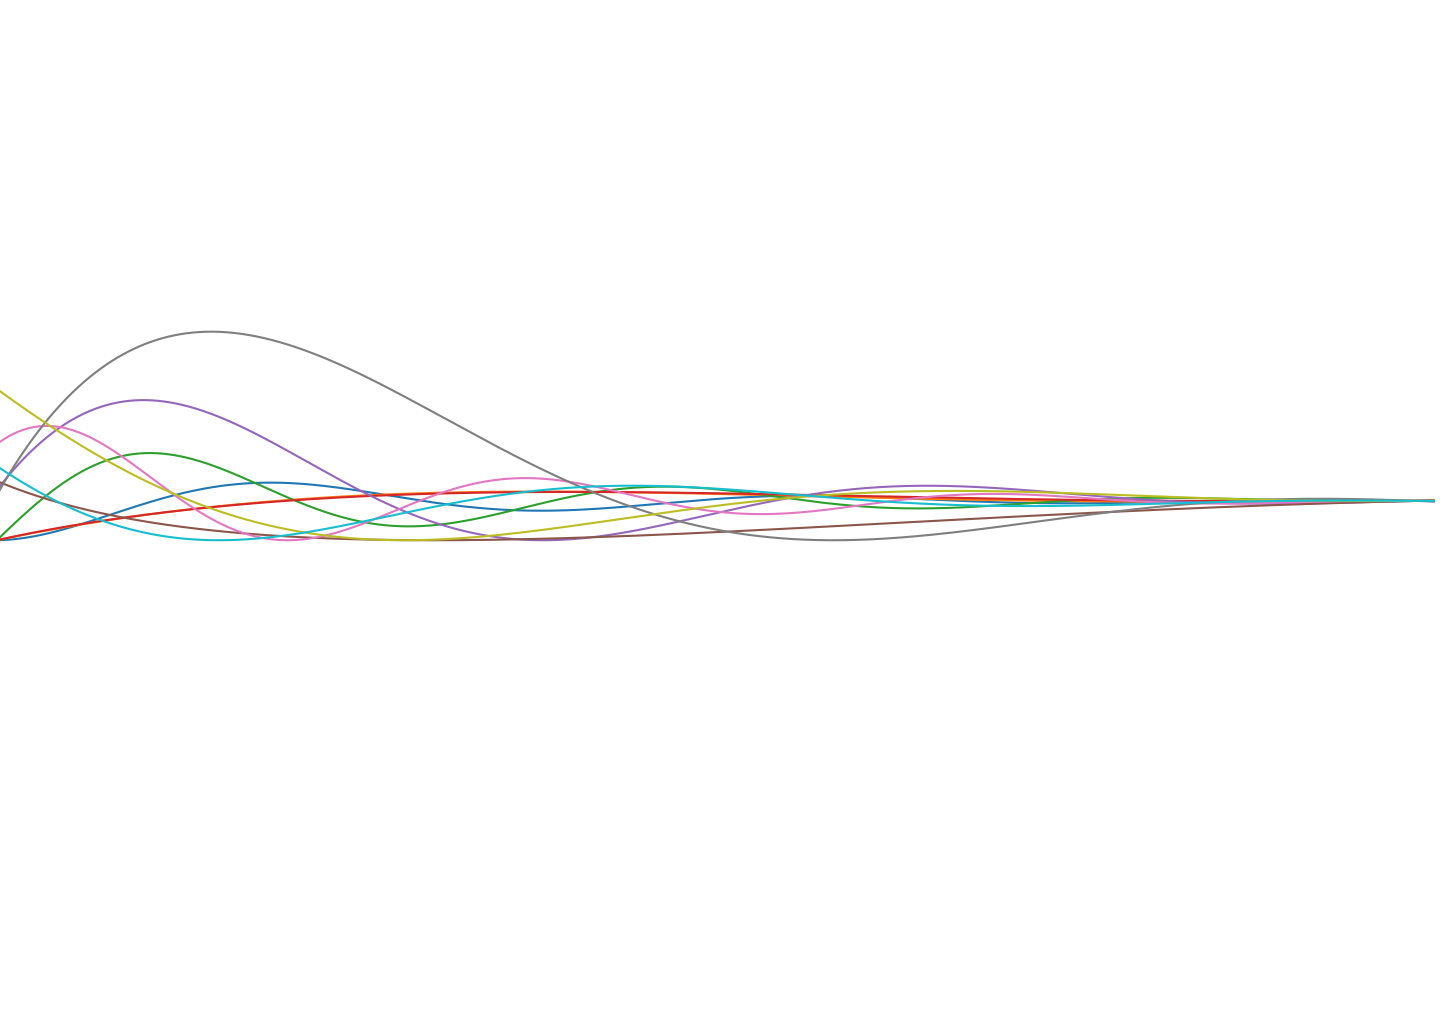
\includegraphics[width=\paperwidth,height=10cm]{header.png}};
    \MakeUppercase{\chaptertitlename}%
        \rlap{ \resizebox{!}{1.5cm}{\thechapter}}
  }
  {10pt}{\Huge}
\titlespacing*{\chapter}{0pt}{-30pt}{-5pt}

%Griffiths' style calligraphy font: use like $\scripty{r}$
\usepackage{calligra}
\DeclareMathAlphabet{\mathcalligra}{T1}{calligra}{m}{n}
\DeclareFontShape{T1}{calligra}{m}{n}{<->s*[2.2]callig15}{}
\newcommand{\scripty}[1]{\ensuremath{\mathcalligra{#1}}}

\begin{document}

\ctikzset{bipoles/length=.6cm}
\newcommand\esymbol[1]{\begin{circuitikz}
\draw (0,0) to [#1] (1,0); \end{circuitikz}}

\title{STK-IN4300 Mandatory Assignment 1}
\author{Gabriel Sigurd Cabrera}

\maketitle

\begin{multicols*}{2}

\section*{Problem 1}

In this exercise, we will be performing a comparison of regression methods on a dataset provided by the \textit{European Bioinformatics Institute} at \url{https://www.ebi.ac.uk/arrayexpress/experiments/E-GEOD-12288/}.  We will be exploring \textit{\textsc{lasso}} and ridge methods for a selection of hyperparameter ($\lambda$) values; with the help of visual aides, we will compare and contrast the dependency of the \textit{mean squared error} (or $MSE$) on $\lambda$, in order to gauge the models' relative efficacies.

The dataset we will be working with is comprised of an input array $\mathbf{X} \in \mathbb{R}^{222 \times 22283}$ with corresponding outputs $\mathbf{y} \in \mathbb{R}^{222}$; to analyze this data, a \texttt{python} script\footnote{Available in the \textbf{Appendix}.} was used in conjunction with the \texttt{rpy2}, \texttt{NumPy}, \texttt{multiprocessing}, and \texttt{sklearn} modules.  The data is normalized as follows:

\begin{equation*}
\mathbf{x}_\text{norm} = \frac{\mathbf{x} - \text{mean}(\mathbf{x})}{\text{std}(\mathbf{x})}
\end{equation*}

Using \texttt{sklearn}, implementing the \textsc{lasso} and ridge algorithms is simple; in Figure \ref{fig_1} we can see that each method's $MSE$ behaves differently as a function of the hyperparameter:

\begin{figure}[H]
	\centering  
	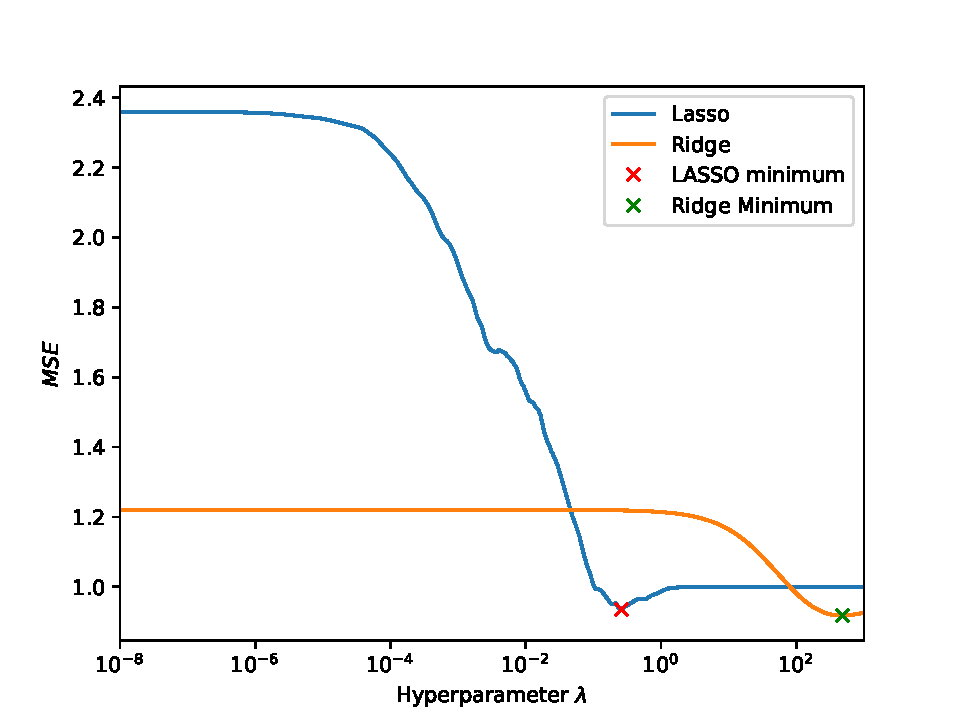
\includegraphics[width = 0.5\textwidth, center]{../a.pdf}
	\caption{The $MSE$ as a function of $\lambda$ for a 1-D polynomial regression using the \textsc{lasso} and ridge algorithms.}
	\label{fig_1}
\end{figure}

We see that the $MSE$ for \textsc{lasso} is consistently superior to the ridge's $MSE$, for all hyperparameters in the selected range.  

This is likely due to the fact that the \texttt{lasso} algorithm is allowed to iterate one-thousand times before breaking the convergence loop; we see further proof in Figure \ref{fig_2}, where the maximum number of iterations was set to five:

\begin{figure}[H]
	\centering  
	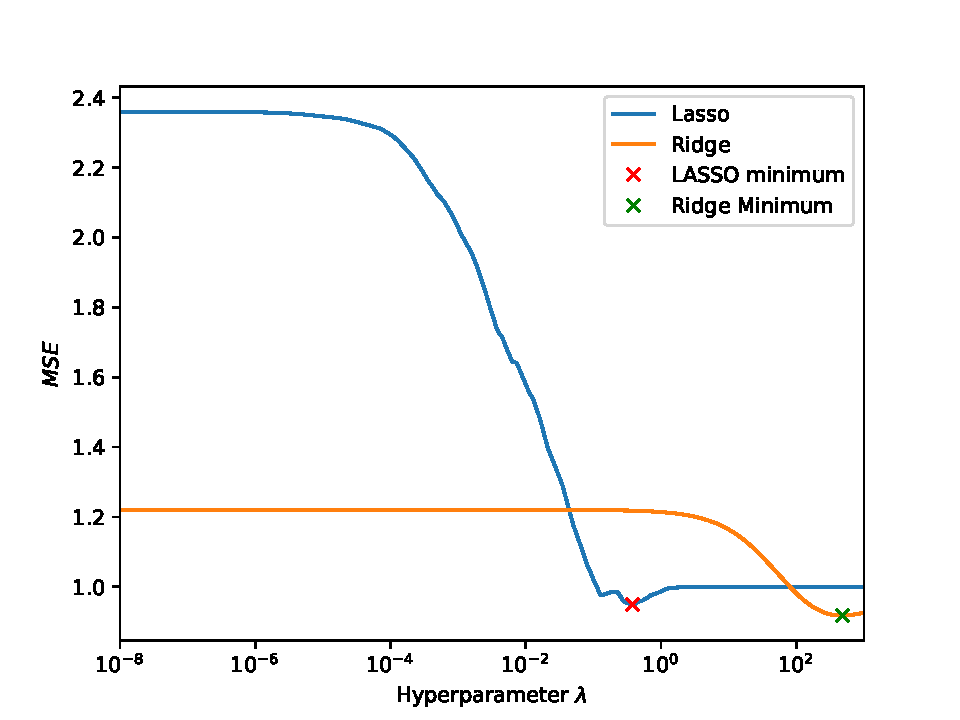
\includegraphics[width = 0.5\textwidth, center]{../a_5_iter.pdf}
	\caption{The $MSE$ as a function of $\lambda$ for a 1-D polynomial regression using the \textsc{lasso} and ridge algorithms; with five \textsc{lasso} iterations.}
	\label{fig_2}
\end{figure}

Here, we see that \textsc{lasso} is not consistently better than ridge, and that it is only competitive for $\lambda $

\section*{Problem 2}

We are given the \textit{linearized} expression for the \textit{object function}:

\begin{equation}
\label{eq_0}
A \equiv \sum_{i=1}^{N} g^\prime(\mathbf{w}_\text{old}^\textsc{t} \mathbf{x}_i)^2 \left( \frac{y_i - g(\mathbf{w}_\text{old}^\textsc{t} \mathbf{x}_i)}{g^\prime(\mathbf{w}_\text{old}^\textsc{t} \mathbf{x}_i)} + \mathbf{w}_\text{old}^\textsc{t} \mathbf{x}_i - \mathbf{w}^\textsc{t} \mathbf{x}_i \right)^2
\end{equation}

Where $y_i, g, g^\prime \in \mathbb{R}$; we also have that $\mathbf{w}, \mathbf{w}_\text{old}, \mathbf{x}_i \in \mathbb{R}^{p \times 1}$ for $i = 1,2,...,N$.  In a practical sense, $N$ might represent the number of points in a dataset, with $p$ representing the number of features present in said dataset.

We are interested in minimizing the scalar-valued $A$; to accomplish this, we must take the derivative of $A$ with respect to $\mathbf{w}$. We will then set this derivative to zero, and solve for the smallest possible $\mathbf{w}$; we will call this value $\mathbf{w}_\text{min}$.

To accomplish this, we must redefine (\ref{eq_0}) such that its \textit{summation notation} is replaced with a \textit{vector/matrix} expression; we begin by redefining some terms.  

\begin{table}[H]
\center
\begin{tabular}{c}
$\mathbf{x}^\textsc{t} \equiv \begin{bmatrix} \mathbf{x}_1 & \mathbf{x}_2 & \cdots & \mathbf{x}_\textsc{n} \end{bmatrix}$ \\ \\
$p_i \equiv \frac{y_i - g(\mathbf{w}_\text{old}^\textsc{t} \mathbf{x}_i)}{g^\prime(\mathbf{w}_\text{old}^\textsc{t} \mathbf{x}_i)} + \mathbf{w}_\text{old}^\textsc{t} \mathbf{x}_i$ \\ \\
$\mathbf{p} \equiv \begin{bmatrix} p_1 & p_2 & \cdots & p_\textsc{n} \end{bmatrix}$ \\ \\
$q_i \equiv g^\prime(\mathbf{w}_\text{old}^\textsc{t} \mathbf{x}_i)^2$ \\ \\
$\mathbf{q} \equiv \begin{bmatrix} q_1 & q_2 & \cdots & q_\textsc{n} \end{bmatrix}$ \\ \\
$\mathbf{r} \equiv \text{diag}(\mathbf{q})^2$
\end{tabular}
\end{table}

This gives us\footnote{This can be verified to be true programmatically – see the \textbf{Appendix}.}

\begin{equation}
\label{eq_1}
A = \sum_{i=1}^{N} q_i ( p_i - \mathbf{w}^\textsc{t} \mathbf{x}_i )^2 = (\mathbf{p} - \mathbf{w}^\textsc{t} \mathbf{x}^\textsc{t}) \mathbf{r} (\mathbf{p} - \mathbf{w}^\textsc{t} \mathbf{x}^\textsc{t})^\textsc{t}
\end{equation}

We then expand the above, giving us several easily-differentiable terms:

\begin{equation*}
A = \mathbf{p} \mathbf{r} \mathbf{p}^\textsc{t} - \mathbf{p} \mathbf{r} \mathbf{x} \mathbf{w} - \mathbf{w}^\textsc{t} \mathbf{x}^\textsc{t} \mathbf{r} \mathbf{p}^\textsc{t} + \mathbf{w}^\textsc{t} \mathbf{x}^\textsc{t} \mathbf{r} \mathbf{x} \mathbf{w}
\end{equation*}

Since each term is a scalar, it is valid to replace each of them with their own transpose if need be. Consider the fact that $\mathbf{w}^\textsc{t} \mathbf{x}^\textsc{t} \mathbf{r}^\textsc{t} \mathbf{p}^\textsc{t} = (\mathbf{p} \mathbf{r} \mathbf{x} \mathbf{w})^\textsc{t}$; since $\mathbf{r}$ is a \textit{diagonal} matrix, we have that $\mathbf{r} = \mathbf{r}^\textsc{t}$, and so we can combine some terms:

\begin{equation*}
A = \mathbf{p} \mathbf{r} \mathbf{p}^\textsc{t} - 2 \mathbf{p} \mathbf{r} \mathbf{x} \mathbf{w} + \mathbf{w}^\textsc{t} \mathbf{x}^\textsc{t} \mathbf{r} \mathbf{x} \mathbf{w}
\end{equation*}

Next, we differentiate with respect to $\mathbf{w}$, keeping in mind the rule $\nabla_\mathbf{x} \mathbf{x}^\textsc{t} \mathbf{v} \mathbf{x} = 2 \mathbf{v} \mathbf{x}$ for $\mathbf{v}$ independent of $\mathbf{x}$:

\begin{equation*}
\nabla_\mathbf{w} A = - 2 \mathbf{p} \mathbf{r} \mathbf{x} + 2 \mathbf{x}^\textsc{t} \mathbf{r} \mathbf{x} \mathbf{w}
\end{equation*}

Setting the above equal to zero allows us to minimize $\mathbf{w}$:

\begin{equation*}
0 = - 2 \mathbf{p} \mathbf{r} \mathbf{x} + 2 \mathbf{x}^\textsc{t} \mathbf{r} \mathbf{x} \mathbf{w}_\text{min}
\end{equation*}

Finally in (\ref{eq_2}), we are left with our desired result:

\begin{equation}
\label{eq_2}
\mathbf{w}_\text{min} = ( \mathbf{x}^\textsc{t} \mathbf{r} \mathbf{x} )^{-1} ( \mathbf{p} \mathbf{r} \mathbf{x} )
\end{equation}

\newpage
\section*{Appendix}

\subsection*{Problem 1}

The program used to calculate and plot the $MSE$ is given below:

\begin{lstlisting}[showstringspaces=false,language=Python,numbers=none]
from sklearn.preprocessing import PolynomialFeatures as Poly
from sklearn.model_selection import train_test_split
from sklearn.linear_model import Lasso, Ridge
from sklearn.preprocessing import normalize
from sklearn.model_selection import KFold
import rpy2.robjects as robjects
from multiprocessing import Pool
import matplotlib.pyplot as plt
import numpy as np

from warnings import filterwarnings
filterwarnings('ignore')

def calculate(data):
    MSE_lasso_step = []
    MSE_ridge_step = []
    a = data[0]
    max_iter = data[1]

    for X_train, X_test, y_train, y_test in data[2]:

        lasso = Lasso(alpha = a, max_iter = max_iter)
        lasso.fit(X_train, y_train)

        ridge = Ridge(alpha = a)
        ridge.fit(X_train, y_train)

        y_lasso = lasso.predict(X_test)
        y_ridge = ridge.predict(X_test)

        MSE_lasso_step.append(np.mean((y_lasso - y_test)**2))
        MSE_ridge_step.append(np.mean((y_ridge - y_test)**2))

    return np.mean(MSE_lasso_step), np.mean(MSE_ridge_step)

robjects.r['load']("data_o1.rdata")
X = np.array(robjects.r['X'])
y =  np.array(robjects.r['y'])

X = (X - np.mean(X))/np.std(X)
y = (y - np.mean(y))/np.std(y)

k = 10
degree = 1
N = 1E3
alphas = np.logspace(-8, 3, N)
max_iter_vals = [5, 1000]
filenames = ["a_5_iter", "a"]

kf = KFold(n_splits = k)
sets = []
poly = Poly(degree = degree)
for train_index, test_index in kf.split(X):
    sets.append((poly.fit_transform(X[train_index]),
    poly.fit_transform(X[test_index]), y[train_index], y[test_index]))

for max_iter, filename in zip(max_iter_vals, filenames):

    MSE_lasso = np.zeros_like(alphas)
    MSE_ridge = np.zeros_like(alphas)

    pool = Pool()
    n = 0
    for i in pool.imap(calculate, ([alphas[j], max_iter, sets] for j in range(int(N)))):
        MSE_lasso[n], MSE_ridge[n] = i
        n += 1
        print(f"\r{100*n/len(alphas):.2f}", end = "")
    print()

    argmin_lasso = np.argmin(MSE_lasso)
    argmin_ridge = np.argmin(MSE_ridge)

    print(f"LASSO lambda = {alphas[argmin_lasso]}, MSE = {MSE_lasso[argmin_lasso]}")
    print(f"Ridge lambda = {alphas[argmin_ridge]}, MSE = {MSE_ridge[argmin_ridge]}")

    plotfunc = plt.semilogx

    plotfunc(alphas, MSE_lasso, "b-", label = "LASSO")
    plotfunc(alphas, MSE_ridge, "r-", label = "Ridge")
    plotfunc([alphas[argmin_lasso]], [MSE_lasso[argmin_lasso]], "bx", label = "LASSO minimum")
    plotfunc([alphas[argmin_ridge]], [MSE_ridge[argmin_ridge]], "rx", label = "Ridge Minimum")
    plt.xlabel("Hyperparameter $\\lambda$")
    plt.ylabel("$MSE$")
    plt.legend()
    plt.xlim([np.min(alphas), np.max(alphas)])
    plt.savefig(f"{filename}.png", dpi = 250)
    plt.close()
\end{lstlisting}

\subsection*{Problem 2}

We can use \texttt{python} to verify that (\ref{eq_1}) holds; below is a script that will generate ten-thousand sets of randomly shaped arrays containing random values – these sets consist of the matrix $\mathbf{x}$, and vectors $\mathbf{w}$, $\mathbf{p}$, and $\mathbf{q}$.  Using the \texttt{NumPy} and \texttt{multiprocessing} modules, we calculate the difference between the values calculated by both sides of (\ref{eq_1}) for each set of initial conditions.

\begin{lstlisting}[showstringspaces=false,language=Python,numbers=none]
from multiprocessing import Pool
import numpy as np

np.random.seed(123)

def test(dummy):
    N = np.random.randint(5, 50)    # Number of datapoints
    p = np.random.randint(2, 6)     # Number of features
    X = np.random.random((N,p))     # Matrix x
    W = np.random.random((p,1))     # Vector w
    P = np.random.random((1,N))     # Vector p
    Q = np.random.random((1,N))     # Vector q

    # Evaluating the summation form
    summation_total = 0
    for i in range(N):
        x_i = X[i,:,np.newaxis]     # Vector x_i
        summation_total += (Q[:,i]**2)*((P[:,i] - W.T @ x_i)**2)

    root_R = np.zeros((N,N))
    for i in range(N):
        root_R[i,i] = Q[:,i]
    R = root_R @ root_R             # Matrix r

    # Evaluating the vector form
    vector_total = (P - W.T @ X.T) @ R @ (P - W.T @ X.T).T

    # Calculating and saving the difference between each total
    difference = np.squeeze(np.abs(summation_total - vector_total))
    return difference

N_tests = 1E4

# Running tests a total of "N_tests" times
pool = Pool()
results = np.array(pool.map(test, (None for i in range(int(N_tests)))))

# Gathering information on the results and printing
max_res, mean_res, median_res = \
np.max(results), np.mean(results), np.median(results)
print("Information on differences between summation total and vector total")
print(f"\tMaximum: {max_res}\n\tMean: {mean_res}\n\tMedian: {median_res}")
\end{lstlisting}

The output is as follows:

\begin{terminal}

Information on differences between summation total and vector total
	Maximum: 1.0658141036401503e-14
	Mean: 5.56243939797696e-16
	Median: 1.1102230246251565e-16
\end{terminal}

Clearly, the only differences are due to numerical error; our assertion that (\ref{eq_1}) holds is therefore near-certain to be true.

\end{multicols*}

\end{document}
